\documentclass{beamer}
\usepackage[utf8]{inputenc}
\usepackage{tikz}
\usepackage{graphicx}
\usepackage{amsmath}
\title{\textbf{Solving 2D Geometry problems using Matrices}}
\author{\textbf{Shaik Mastan, J.Prabhath, K.Srikanth}}
\date{February 14, 2019}
\usetheme{Frankfurt}
\begin{document}
\maketitle
\begin{frame}
\frametitle{\textbf{Theory}}
\begin{itemize}
\item The equation of a line passing through a point 'A' and normal to a vector 'n', in matrix form is$-$\centering \begin{equation}
    n^T(x - A) = 0
\end{equation}
\item The foot of the perpendicular drawn from the centre of a circle onto any chord is the mid$-$point of the chord.\newline Conversely, the line joining the centre of a circle and the midpoint of a chord is perpendicular to the chord.\newline
\item The solution of the linear equations defined by Ax = b (where A is invertible),is 
\begin{equation}x = A^{-1}b
\end{equation}
\end{itemize}
\end{frame}
\section{Question}
\begin{frame}
\frametitle{\textbf{Problem}}
A circle passes through the points \begin{bmatrix}
2\\
3
\end{bmatrix} and \begin{bmatrix}
4\\
5
\end{bmatrix}. If its centre lies on the line \begin{bmatrix}
-1 & 4
\end{bmatrix}x + 3 = 0, find its radius.
\end{frame}
\section{Diagram}
\begin{frame}
\frametitle{\textbf{Schematic Diagram}}
\setlength{\unitlength}{0.25cm}
\thicklines
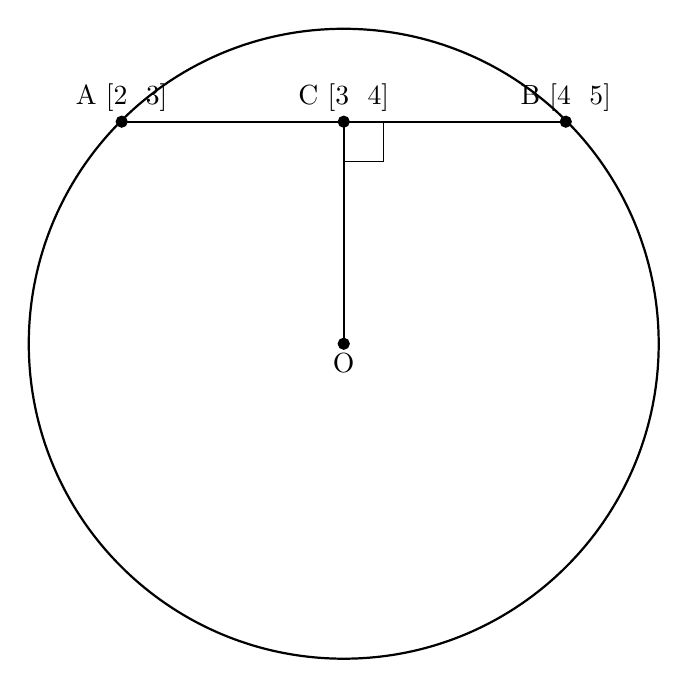
\begin{tikzpicture}
\centering
\draw[black, thick] (0, 0) circle(4.0);
\draw[black, thick] (-2.82, 2.82) -- (2.82, 2.82);
\filldraw[black] (0, 2.82) circle (2pt) node[anchor=south] {C [3 \ 4]};
\filldraw[black] (-2.82, 2.82) circle (2pt) node[anchor=south] {A [2 \ 3]};
\filldraw[black] (2.82, 2.82) circle (2pt) node[anchor=south] {B [4 \ 5]};
\draw[black, thick] (0, 0) -- (0, 2.82);
\filldraw[black] (0, 0) circle (2pt) node[anchor = north] {O};
\draw (0, 2.82) rectangle (0.5, 2.32);
\end{tikzpicture}
\end{frame}
\section{Solution}
\begin{frame}
\frametitle{\textbf{Theoretical solution}}
Let A = \begin{bmatrix}
2 \\ 
3
\end{bmatrix} and B = \begin{bmatrix}
4 \\ 
5\end{bmatrix}. Let the centre of the circle be O.
The mid-point of the chord AB is C = $\frac{(A + B)}{2}$ = \begin{bmatrix}
3\\
4
\end{bmatrix}
\newline Let AB = B - A (direction vector),
\newline which gives AB = \begin{bmatrix}
2 & 2
\end{bmatrix}\newline
From the stated theory, the line joining C and O is normal to the chord AB. The equation of OC is thus -
\begin{equation}
    AB^T(x - C) = 0.\end{equation} which gives,\centering \begin{bmatrix}
    2 & 2
    \end{bmatrix}x = 14.
\end{frame}
\begin{frame}
It is given that the centre of the circle lies on the line\newline\centering $$ [-1 \ 4]x + 3 = 0.$$\newline\newline The centre is the point of intersection of OC and $$ [-1 \ 4]x + 3 = 0. $$
Let P = 
\begin{bmatrix}
-1 & 4 \\ 
2 & 2
\end{bmatrix}. Writing the equations in matrix form, we get\newline 
\centering P x = \begin{bmatrix}
-3\\
14
\end{bmatrix}.\begin{equation} x = P^{-1}b\end{equation}$(since \ P \ is \ invertible.)$
x = $ \frac{1}{10}$\begin{bmatrix}
-2 & 4\\
2 & 1
\end{bmatrix}\begin{bmatrix}
-3\\
14
\end{bmatrix},
x = \begin{bmatrix}
6.2\\
0.8
\end{bmatrix}
\end{frame}
\begin{frame}
The obtained solution is nothing but 'O'.\newline The radius can be obtained by computing the norm of (O - A) or (O - B).
\newline\newline Radius = $||(O - A)||$ = $||[4.2 \ -2.2]||$ = 4.741 units
\end{frame}
\begin{frame}{\textbf{Plotting}}
\includegraphics[scale = 0.65]{Circle.png}  
\end{frame}
\end{document}
